% 功 功率
% 做功|功率|能量|位移|曲线积分

\pentry{力场\upref{V},矢量的内积\upref{Dot},定积分\upref{DefInt}}

\begin{figure}[ht]
\centering
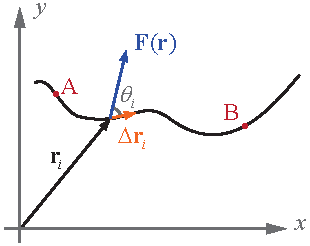
\includegraphics[width=6cm]{./figures/Fwork1.pdf}
\caption{在一小段位移中,把变力看做恒力}\label{Fwork_fig1}
\end{figure}

如\autoref{Fwork_fig1},当质点沿着曲线运动时,有一个力作用在其上, 当质点的位置为 $\bvec r$ 时,力为 $\bvec F(\bvec r)$. 下面求质点从点 $A$ 运动到点 $B$ 的过程中,力对质点的做功.

把从 $A$ 到 $B$ 这段曲线看成由许多小位移 $\Delta \bvec r_1, \Delta \bvec r_2 \dots \Delta \bvec r_n$ 组成, 对其中第 $i$ 个进行分析. 由于 $\Delta \bvec r_i$ 很短,质
点经过 $\Delta \bvec r_i$ 的过程中位矢 $\bvec r$ 几乎不变,记为常矢量 $\bvec r_i$. 在这小段中,  $\bvec F(\bvec r)$ 也可以近似看成是恒力 $\bvec F(\bvec r_i)$. 

现在把 $\bvec F(\bvec r_i)$ 分解成垂直于 $\Delta \bvec r_i$ 和平行于 $\Delta \bvec r_i$ 的两个正交分量,其中垂直分量不做功,平行分量的大小为 $ \abs{\bvec F(\bvec r_i)} \cos \theta_i$, 该分量做功大小为
\begin{equation}
\Delta W_i = \abs{\bvec F(\bvec r_i)} \abs{\Delta \bvec r_i} \cos \theta_i
\end{equation}
上式可以表示成矢量内积\upref{Dot}的形式
\begin{equation}\label{Fwork_eq2}
\Delta W_i = \bvec F(\bvec r_i) \vdot \Delta \bvec r_i
\end{equation}
把上式对所有的 $i$ 求和,就得到了做功的近似表达式
\begin{equation}
W_{ab} = \sum_{i = 1}^n \Delta W_i  \approx \sum_{i = 1}^n \bvec F(\bvec r_i) \vdot \Delta \bvec r_i 
\end{equation} 
事实上,当曲线分割的越细,即 $n$ 越大时,上式就越精确地成立.类比定积分\upref{DefInt}中的介绍,令 $n \to \infty $, 把求和符号换成积分符号,把表示增量的 $\Delta $ 换成微分符号 $\dd{}$, 则不等号可以变为等号.
\begin{equation}
W_{ab} = \lim_{n \to \infty } \sum_{i = 1}^n \bvec F(\bvec r_i) \vdot \Delta \bvec r_i  = \int_{C_{ab}} \bvec F(\bvec r) \vdot \dd{\bvec r}
\end{equation} 
不同于一元函数的积分,这一类特殊的积分叫做\textbf{线积分},详见“线积分\upref{IntL}”.

\subsection{力的功率}
\textbf{功率}(瞬时)的定义为做功的变化率,即
\begin{equation}
P = \lim_{\Delta t\to 0} \frac{\Delta W}{\Delta t} = \dv{W}{t}
\end{equation}
根据\autoref{Fwork_eq2},力的功率为
\begin{equation}
P = \lim_{\Delta t\to 0} \frac{\bvec F(\bvec r_i)\vdot\Delta\bvec r_i}{\Delta t_i} = \bvec F \vdot\dv{\bvec r}{t} = \bvec F\vdot\bvec v
\end{equation}






